Apart from the applied density fitting method, the chosen orbital-free basis set arguably has an even greater impact on the accuracy of the density-fitted density. The commonly used even-tempered basis sets are reliable but often inefficient for defining an orbital-free basis. Their simple construction algorithm \cite{const} broadly covers the possible density space without refinement.

To improve the performance of our orbital-free basis set, it is sensible to adopt a basis set with higher resolution in regions where density fluctuates more rapidly. We construct this improved basis by beginning with an even-tempered set and using differentiable integrals and autograd.

\section{Using differentiable integrals to optimize an orbital free basis set}
Given differentiable basis integrals, we can describe the complete density fitting procedere in a completely differentiable way. For a given target density we want to optimize the L2 norm of the fitted density, so we are going to start with the overlap formulation of density ftting defined in \eqref{overlap_eq}. Other formulations using the residual hartree energy can also be easily formulated but they these integrals are much more costly to compute. We also found this formulation to be sufficient to optimize the relevant metrics to an acceptable level.
\begin{align}
    \mathcal{L}[\rho] &= \min_{\rho'}\left(||\rho-\rho'||_{\text{L2}}\right)\\
    & = \min_{\{p_{\mu}\}_{\mu \in 1,...,n_b}} \mathbf{p}W \mathbf{p} - 2 \mathbf{p} \bar L \bar\Gamma + \bar\Gamma \bar D \bar\Gamma\\
    & = \left[\mathbf{p} W \mathbf{p} - 2 \mathbf{p} \bar L \bar\Gamma+ \bar\Gamma \bar D \bar\Gamma\right]_{\mathbf{p} = W^{-1}\bar{L}\bar\Gamma}\\
    & = \bar \Gamma \bar L ^T W^{-1} \bar L \bar \Gamma - 2 \bar \Gamma \bar L^T W^{-1} \bar L \bar \Gamma + \bar \Gamma \bar D \bar \Gamma\\
    & = - \bar \Gamma \bar L^T W^{-1} \bar L \bar \Gamma + \bar \Gamma \bar D \bar \Gamma
\end{align}
We can now insert the dependency of our integrals on the exponents $\{\mathbf{\alpha}_Z\}_{Z\in \text{H,C,N,O,F}}$ for the gaussian basis functions for each atom.
The dependent integrals are the two center integral $W_{\mu,\nu}(\mathbf{\alpha}) = \langle \omega_\mu(\mathbf{\alpha})|\omega_\nu(\mathbf{\alpha})\rangle$
 and the three center overlap integral $L_{\mu,\gamma\sigma}(\mathbf{\alpha}) = \langle \omega_\mu(\mathbf{\alpha})|\eta_\gamma\eta_\sigma\rangle$. The 4 center overlap integral $D$ does not depend on the orbital free basis functions $\omega_\mu(\mathbf{\alpha})$ and can therefor be omitted from the final loss. For a single molecule geometry $\mathcal{M}$ we can define now our loss as
 \begin{align}\label{loss_basis_set_fitting}
    \text{Loss}_\text{molecule}(\mathcal{M}, \Gamma,\mathbf{\alpha}) & = - \bar \Gamma \bar L_{\mathcal{M}}^T(\mathbf{\alpha}) W_{\mathcal{M}}^{-1}(\mathbf{\alpha}) \bar L_{\mathcal{M}}(\mathbf{\alpha}) \bar \Gamma
 \end{align}
The loss of our entire dataset $\{\mathcal{M}_i,\Gamma_i\}_{i\in 1,...,N_{\text{molecules}}}$, containing the atomic structures and ground state densities, amounts to:
\begin{align} \label{loss_dataset_basis_set_fitting}
    \text{Loss}(\{\mathcal{M}_i,\Gamma_i\}_{i\in 1,...,N_{\text{molecules}}},\mathbf{\alpha}) = \sum\limits_{i=1}^{N_{\text{molecules}}} \text{Loss}_\text{molecule}(\mathcal{M}_i, \Gamma_i,\mathbf{\alpha})
\end{align}
For the atomic structures, we used molecules from the popular dataset QM9\ref{QM9}. For the target density, we again used the ground state density of molecules generated by a Kohn-Sham calculation using the PBE exchange-correlation functional and the "6-31G(2df,p)" basis set for the orbitals.
As our entire framework is written in PyTorch and is differentiable, the gradients of the loss in the direction of the individual exponents can be computed using PyTorch's autograd. We then optimize the exponents by minimize our loss function \eqref{loss_dataset_basis_set_fitting} using stochastic gradient descent.
To summarize our training setup:
We perform the entire training loop of building the integrals, computing the loss, and backpropagation on a single GPU. As the integrals require significant RAM (~20GB), we are restricted to a batch size of 1. We trained for approximately 20,000 steps. As the number of steps and parameters (~100) is much smaller than the number of training samples in the dataset (~100,000), we view the risk for overfitting to be very low.
\subsection{Comparison of performance of fitted basis sets with vanilla even-tempered basis sets}
We compare several fitted basis sets originating from even-tempered basis sets with $\beta$ equal to 3 or 2.5 using the same metrics that we used for the different density fitting methods (Section \ref{metrics}). We are going to compare them using the density fitting method hartree+external MOFDFT, which we introduced in the previous chapter \ref{chapter:densityfitting}.
\section{Additional Side Losses}
Using the previously mentioned loss \ref{loss_basis_set_fitting} alone isn't sufficient to guarantee that the fitted basis set produces stable labels. This is evident in the strongly increased standard deviation of some coefficients. In practice, this leads to slower and worse training. The cause of this instability becomes apparent when examining the individual metrics.
To counteract this behavior, we introduce additional side losses on the fitted coefficients $\mathbf{p}(\mathbf{\alpha}) = W^{-1}(\mathbf{\alpha}) \bar L(\mathbf{\alpha}) \bar \Gamma$ during training. These side losses are meant to regularize the exponents by ensuring more stable coefficients. We introduce the following side losses:
 \begin{align}
    \text{Loss}_\text{Coeffs}(\mathcal{M},\mathbf{p}(\mathbf{\alpha})) &= \epsilon_\text{Coeffs}||\mathbf{p}(\mathbf{\alpha})||^2\\
    \text{Loss}_\text{STDCoeffs}(\mathcal{M},\mathbf{p}(\mathbf{\alpha})) &= \epsilon_\text{STDCoeffs}\left\lVert\subset{\text{}}{\text{std}}(\mathbf{p}(\mathbf{\alpha}))\right\rVert^2\\
    \text{Loss}_\text{STDCoeffsDiff}(\mathcal{M},\mathbf{p}(\mathbf{\alpha})) &=\label{sideloss3}\\ \nonumber\epsilon_\text{STDCoeffs}\sum\limits_{\text{atom} \mathcal{A}\in \mathcal{M}}\sum\limits_{\text{shell} \mathcal{S}\in \mathcal{A}}&\left\lVert \text{std}(\mathbf{p}(\mathbf{\alpha}))1|_{\mathcal{S}}-\sum\limits_{i=1}^{N_b}\frac{\left(\text{std}(\mathbf{p}(\mathbf{\alpha}))1|_{\mathcal{S}}\right)_i}{||\mathcal{S}||}\right\rVert^2
 \end{align}
The first loss function the size of the individual coefficients, the second loss function regularizes the standart deviation of the coefficients and the third loss function regularizes the difference of standart deviation in each shell of each atom from the mean of each atom. The weights $\epsilon_\text{Coeffs}$, $\epsilon_\text{STDCoeffs}$ and $\epsilon_\text{STDCoeffsDiff}$ are hyperparameters that need to be tuned. $1|_{\mathcal{S}}\in \{0,1\}^{N_b}$ is a binary mask that is 1 for the coefficients of the shell $\mathcal{S}$ and 0 otherwise, while $||\mathcal{S}|| = \sum_i 1|_{\mathcal{S}}_i$ is the number of components of the shell. The standart deviation is computed using A running STD implementation following welfords algorithm \cite{Welford} over the .The loss functions are then added to the loss function \eqref{loss_dataset_basis_set_fitting} and the entire loss is minimized using stochastic gradient descent. In praxis all varirants resulted in smoother coefficients but the third loss \eqref{sideloss3} archived this while disrupting the training the least. Which is why when refering to regularized basis sets we are refering to basis sets that were trained with this loss function and a parameter of $\epsilon_\text{STDCoeffsDiff}=0.001$.\\


\section{Comparison of the different fitted basis sets}
We now compare the performance of different basis sets. As the risk of overfitting is very low and for ease of reproducibility, we compare 9 different basis sets on the first 1000 molecules of QM9. The basis sets include even-tempered basis sets with $\beta = 1.5,2.0,2.5,3.0$, the def2-universal-jfit basis set, fitted basis sets initialized from even-tempered basis sets with $\beta = 2.5,3.0$, and the regularized versions of these basis sets. We compare the different fitted basis sets using the same metrics as before for the different density fitting methods in section \ref{metrics}. To give a sense of the difference in the number of basis functions, we compare the number of basis functions for each angular momentum for each atom type in table \ref{tab:basis-comparison-detailed}. The number of basis functions in the even-tempered basis sets increases with lower $\beta$, as $\beta$ defines the factor between the exponents of successive basis functions in each shell. The lowest and highest exponents of each shell are chosen such that all products of basis functions in the orbital basis set "6-31G(2df,p)" can be represented relatively well. The basis set "def2-universal-jfit" is commonly used to fit the 4-index Hartree tensor and is optimized for this procedure. While the even-tempered basis sets have a single Gaussian per basis function, "def2-universal-jfit" uses contracted Gaussians to form the individual basis functions, which is why it relies on a smaller number of basis functions.\\
\begin{table}
\centering
\tiny
\begin{tabular}{|l|ccc|ccccc|ccccc|ccccc|ccccc|}
\hline
& \multicolumn{3}{c|}{H} & \multicolumn{5}{c|}{C} & \multicolumn{5}{c|}{N} & \multicolumn{5}{c|}{O} & \multicolumn{5}{c|}{F} \\
Basis Set & s & p & d & s & p & d & f & g & s & p & d & f & g & s & p & d & f & g & s & p & d & f & g \\
\hline
even\_tempered\_1.5 & 12 & 7 & 2 & 25 & 17 & 15 & 7 & 4 & 25 & 18 & 15 & 7 & 4 & 25 & 18 & 16 & 7 & 4 & 25 & 18 & 16 & 7 & 4 \\
even\_tempered\_2.0 & 7 & 4 & 1 & 15 & 10 & 9 & 4 & 3 & 15 & 11 & 9 & 4 & 3 & 15 & 11 & 9 & 5 & 3 & 15 & 11 & 9 & 5 & 3 \\
even\_tempered\_2.5 & 6 & 3 & 1 & 11 & 8 & 7 & 3 & 2 & 11 & 8 & 7 & 4 & 2 & 11 & 8 & 7 & 4 & 2 & 11 & 8 & 7 & 4 & 2 \\
even\_tempered\_3.0 & 5 & 3 & 1 & 9 & 7 & 6 & 3 & 2 & 10 & 7 & 6 & 3 & 2 & 10 & 7 & 6 & 3 & 2 & 9 & 7 & 6 & 3 & 2 \\
def2-universal-jfit & 3 & 1 & 1 & 6 & 4 & 3 & 1 & 1 & 6 & 4 & 3 & 1 & 1 & 6 & 4 & 3 & 1 & 1 & 6 & 4 & 3 & 1 & 1 \\
fitted basis 2.5 & 6 & 3 & 1 & 11 & 8 & 7 & 3 & 2 & 11 & 8 & 7 & 4 & 2 & 11 & 8 & 7 & 4 & 2 & 11 & 8 & 7 & 4 & 2 \\
fitted reg. basis 2.5 & 6 & 3 & 1 & 11 & 8 & 7 & 3 & 2 & 11 & 8 & 7 & 4 & 2 & 11 & 8 & 7 & 4 & 2 & 11 & 8 & 7 & 4 & 2 \\
fitted basis 3.0 & 5 & 3 & 1 & 9 & 7 & 6 & 3 & 2 & 10 & 7 & 6 & 3 & 2 & 10 & 7 & 6 & 3 & 2 & 9 & 7 & 6 & 3 & 2 \\
fitted reg basis 3.0 & 5 & 3 & 1 & 9 & 7 & 6 & 3 & 2 & 10 & 7 & 6 & 3 & 2 & 10 & 7 & 6 & 3 & 2 & 9 & 7 & 6 & 3 & 2 \\
\hline
\end{tabular}
\caption{Detailed comparison of irreducible representations for different basis sets. For each atom, the number of basis functions is shown for each angular momentum (s, p, d, f, g). Hydrogen only includes s, p, and d functions. Each number represents the count of basis functions for that specific angular momentum. \footnote{Formatting done by claude}}
\label{tab:basis-comparison-detailed}
\end{table}
We are going to start by comparing the energies produced by the different basis sets, which are shown in figure \ref{fig:AE_energies_basis_sets}. First of all we notice that for the even tempered basis sets the ones with a higher number of basis functions perform consistently better than the ones with a lower number of basis functions for all fitted energies. "def2-universal-jfit" performs very poorly on account of its low number of basis functions. The fitted basis sets also produce consistenly more accurate energies than the even tempered basis set they originated from, often beating even tempered basis sets with a higher number of basis functions. The regularized basis sets perform slightly worse than the non regularized basis sets. \\
\begin{figure}
    \centering
    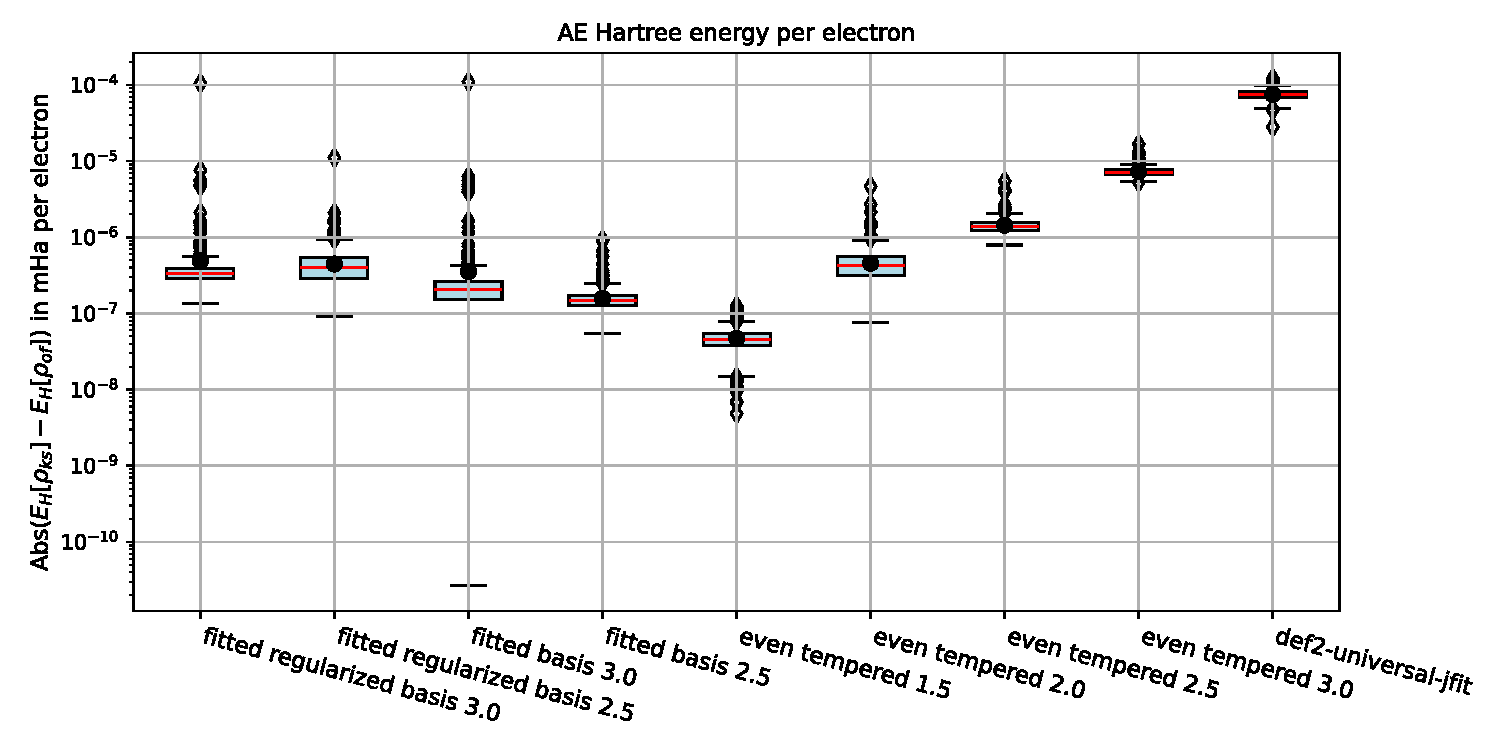
\includegraphics[width=0.75\textwidth]{chapters/results/results_images/AE_hartree_energy_on_hartree+external_MOFDFT_for_different_basis_sets}
    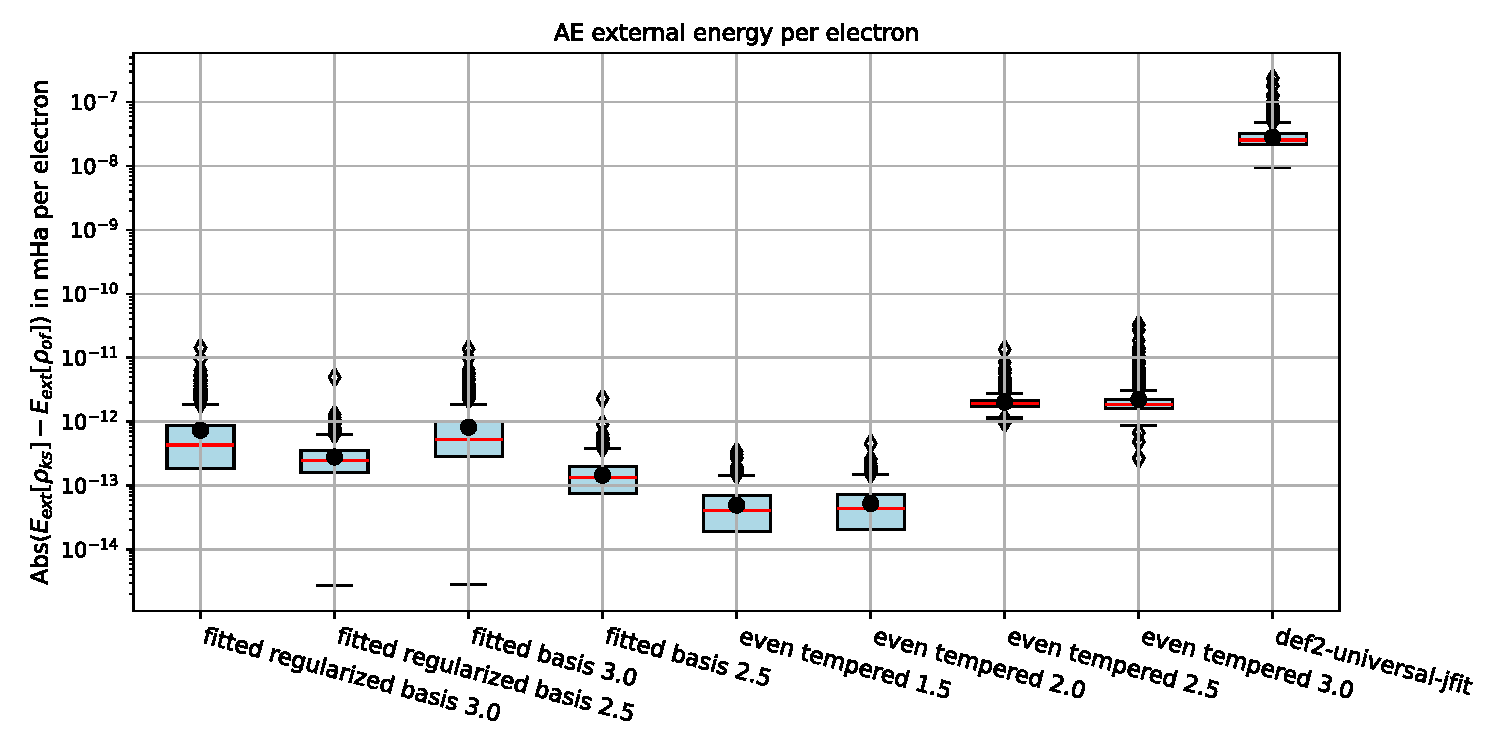
\includegraphics[width=0.75\textwidth]{chapters/results/results_images/AE_ext_energy_on_hartree+external_MOFDFT_for_different_basis_sets}
    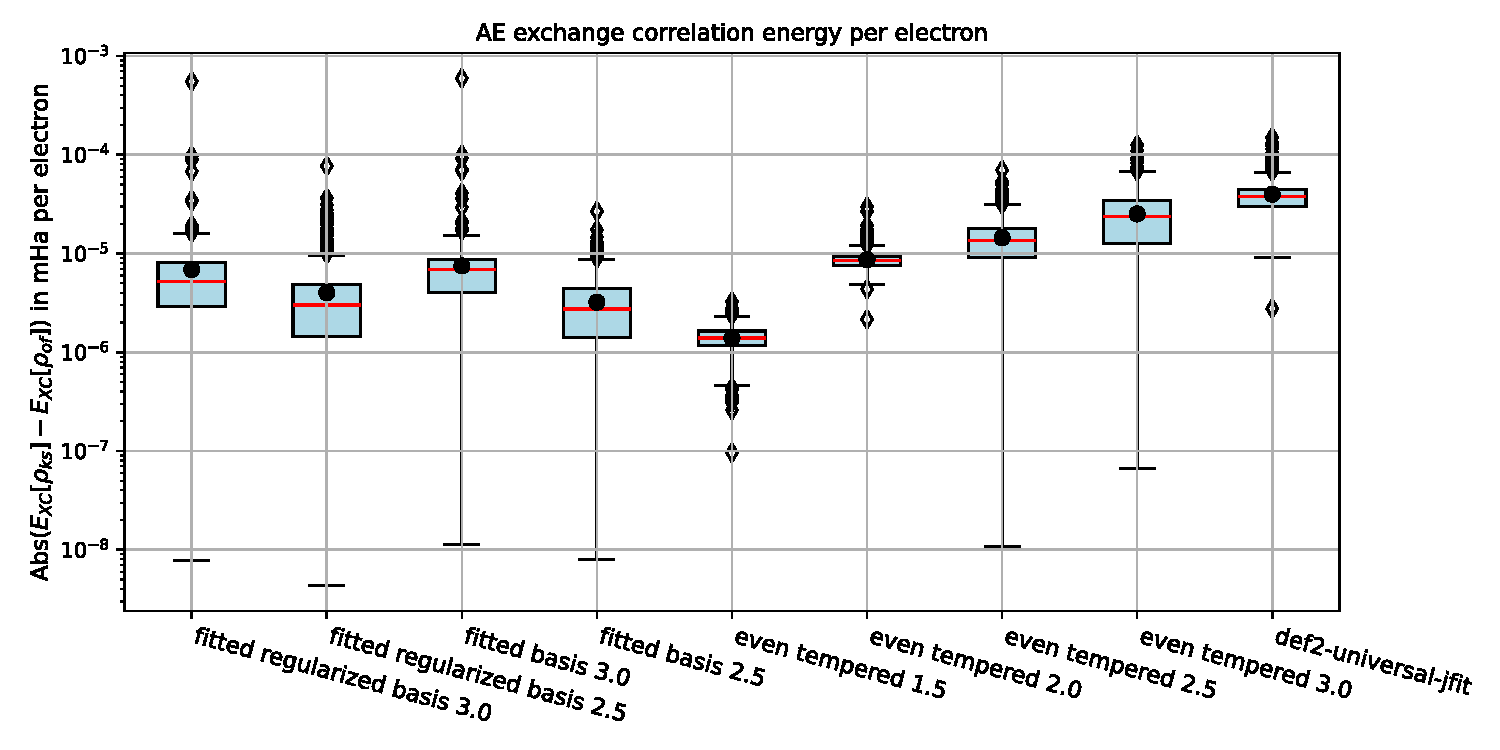
\includegraphics[width=0.75\textwidth]{chapters/results/results_images/AE_xc_energy_on_hartree+external_MOFDFT_for_different_basis_sets}
    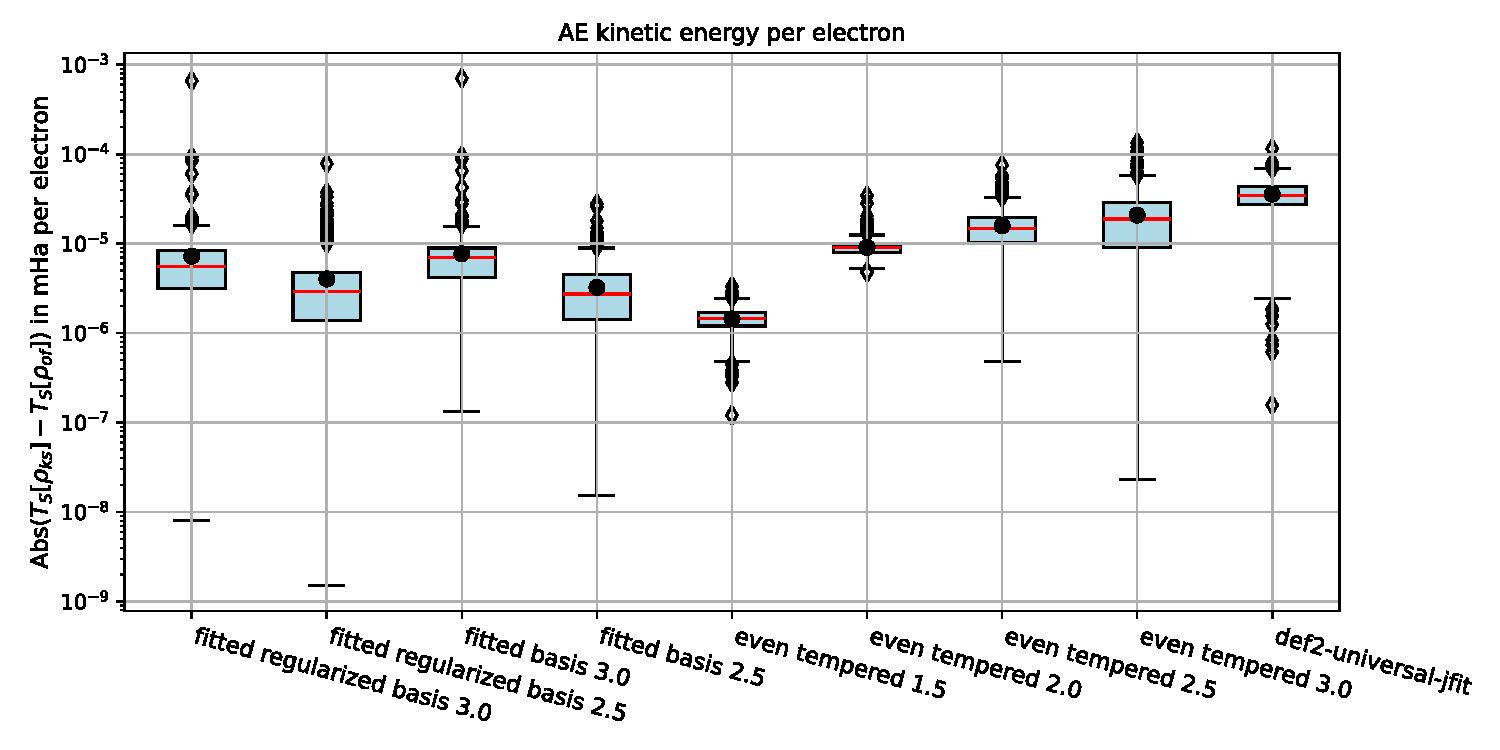
\includegraphics[width=0.75\textwidth]{chapters/results/results_images/AE_kin_energy_on_hartree+external_MOFDFT_for_different_basis_sets}
    \caption{Boxplots(\ref{boxplots}) of the AE for the different energies on the fitted basis sets averaged over the first 1000 molecules of QM9} \label{fig:AE_energies_basis_sets}
\end{figure}
If we now take a look at the difference in densities in figure \ref{fig:density_error_basis_sets} we can see similar results. The bigger even tempered basis sets outperform the smaller ones and the fitted basis sets outperform their respective fitted basis functions. "def2-universal-jfit" performs poorly in comparison, but on account of its contracted basis functions it still performs almost as well as even tempered 3.0 while having a much lower number of basis functions.\\
The additional metrics in figure \ref{fig:density_error_basis_sets} show that most basis sets have a relatively low number of negative densities which should be of not much concern. Only the fitted basis set with $\beta = 3.0$ and its fitted variant as well as "def2-universal-jfit" have a few outlier which have a higher number of negative densities. The maximal absolute gradient is also very consitent over all basis sets.\\
\begin{figure}
    \centering
        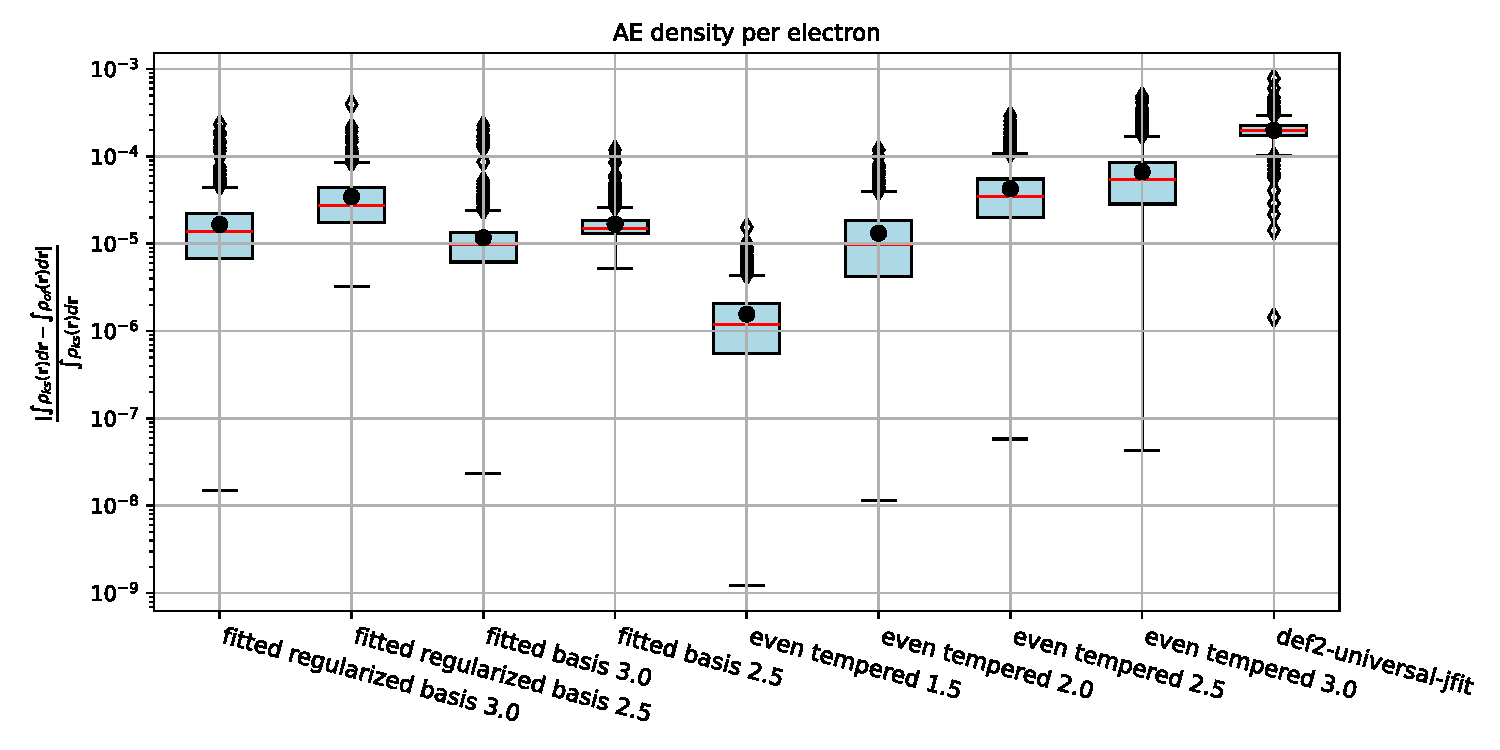
\includegraphics[width=0.75\textwidth]{chapters/results/results_images/AE_density_on_hartree+external_MOFDFT_for_different_basis_sets}
    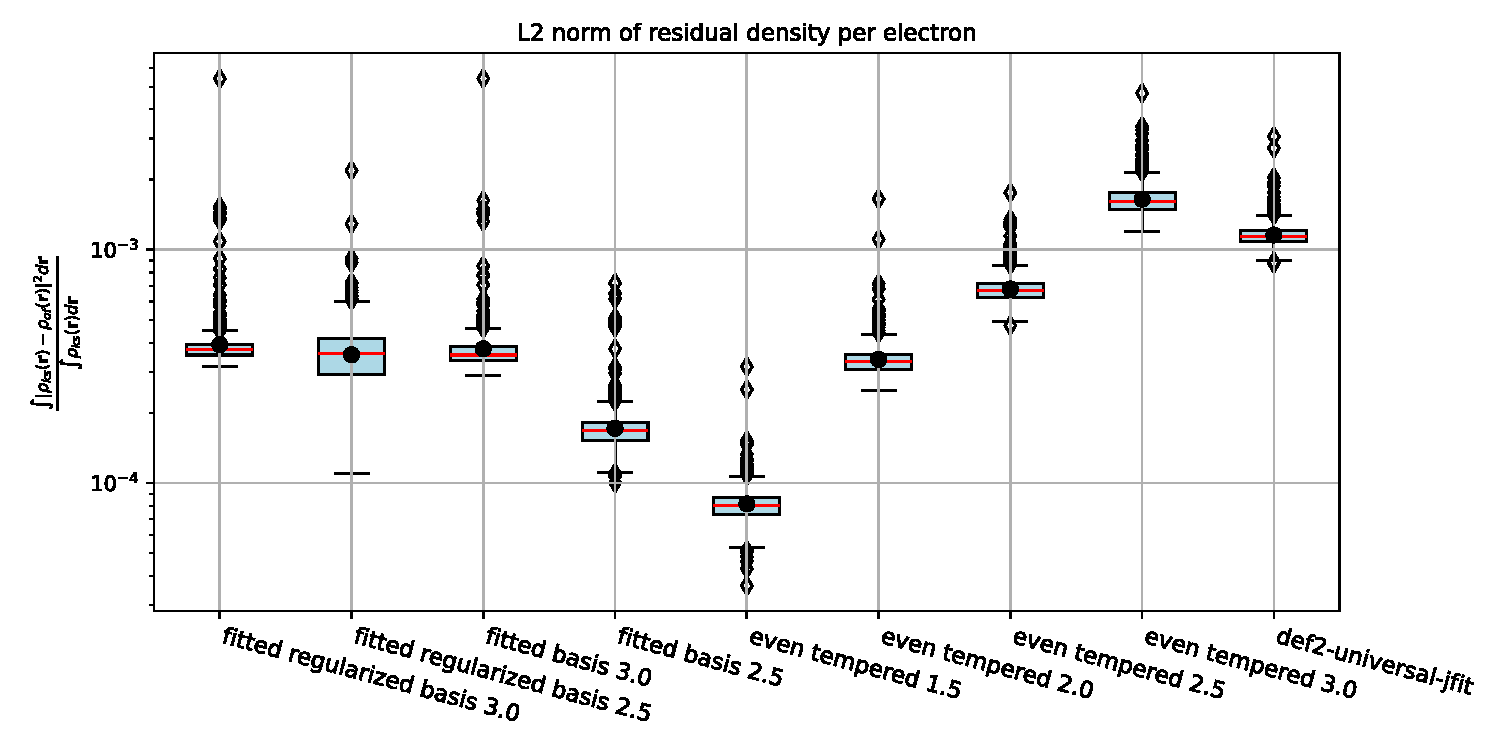
\includegraphics[width=0.75\textwidth]{chapters/results/results_images/L2_residual_densities_on_hartree+external_MOFDFT_for_different_basis_sets}
    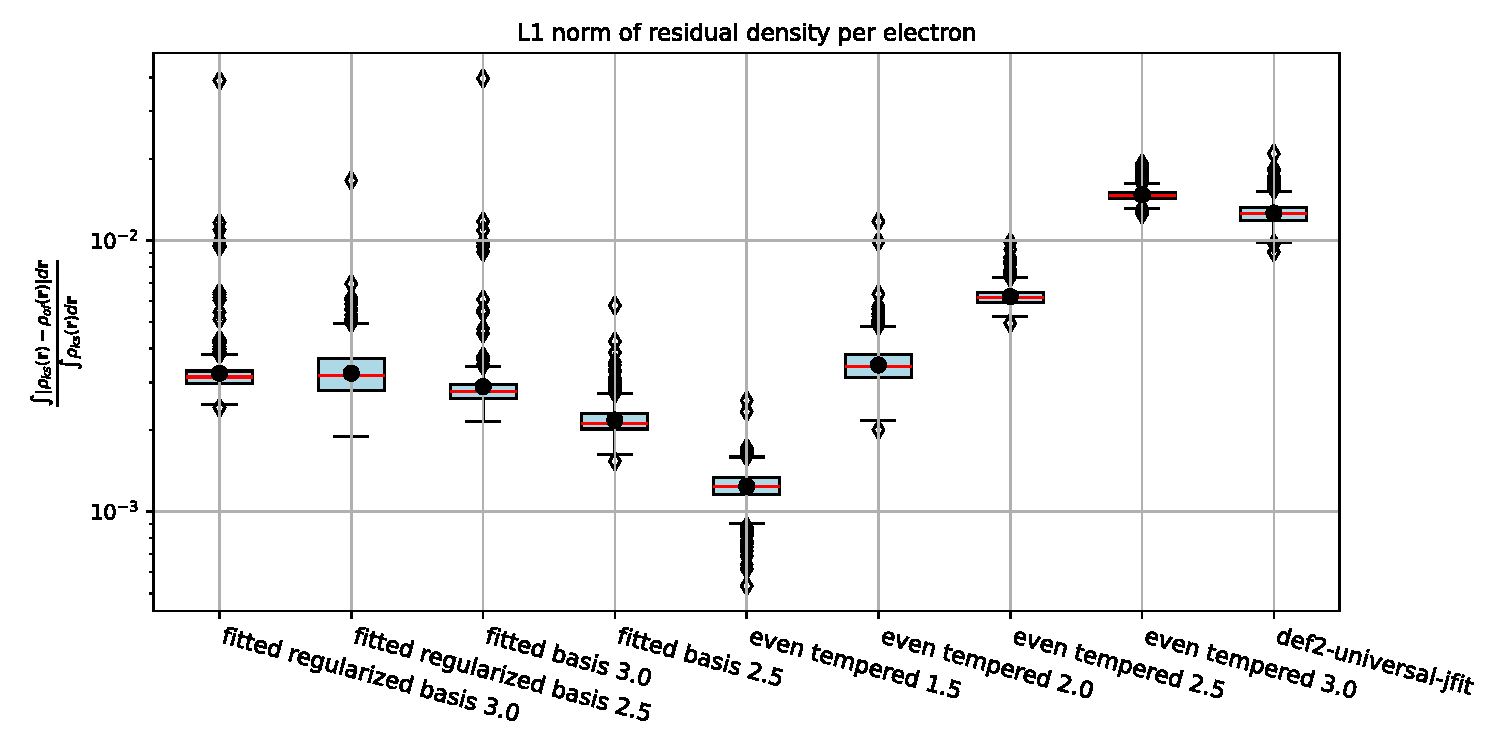
\includegraphics[width=0.75\textwidth]{chapters/results/results_images/L1_residual_densities_on_hartree+external_MOFDFT_for_different_basis_sets}
    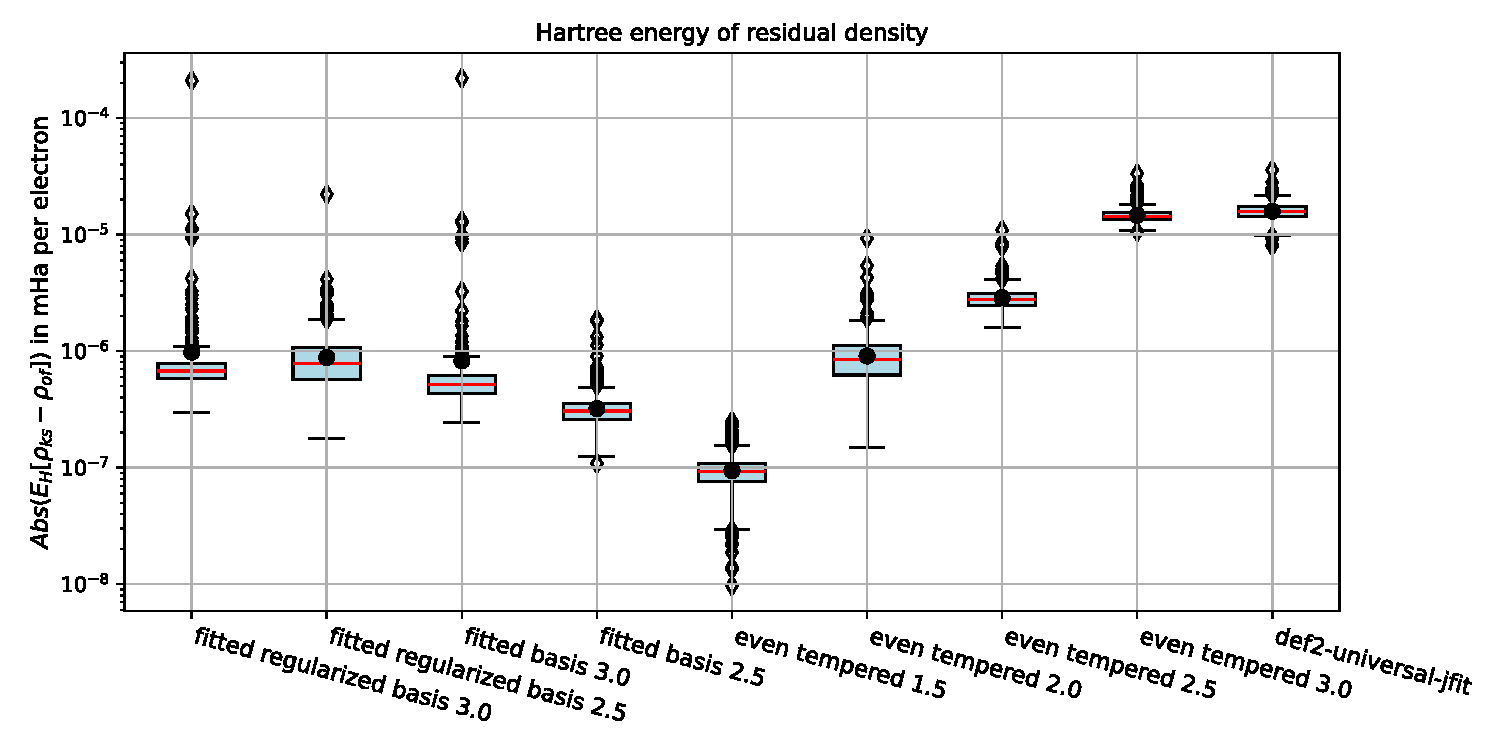
\includegraphics[width=0.75\textwidth]{chapters/results/results_images/L2_residual_hartree_on_hartree+external_MOFDFT_for_different_basis_sets}
\caption{Boxplots(\ref{boxplots}) comparing the error in density fitting for the different basis sets over the first 1000 molecules of QM9} \label{fig:density_error_basis_sets}
\end{figure}
In the third plot we depicted the variance of the individual basis functions at each atomtype. For the even tempered basis functions the ones with a higher number of basis functions have a larger standart deviation on average. The fitted basis functions seem
 to have a higher end of exponents than their vanilla counterparts. An explaination for the this behavior we can find in figure \ref{fig:var_coeffseven_tempered_3.0}- \ref{fig:var_coeffsfitted_regularized_basis_3.0}: Here we plotted the mean and standart deviation of the distinct coefficients.
    \begin{figure}
    \centering
    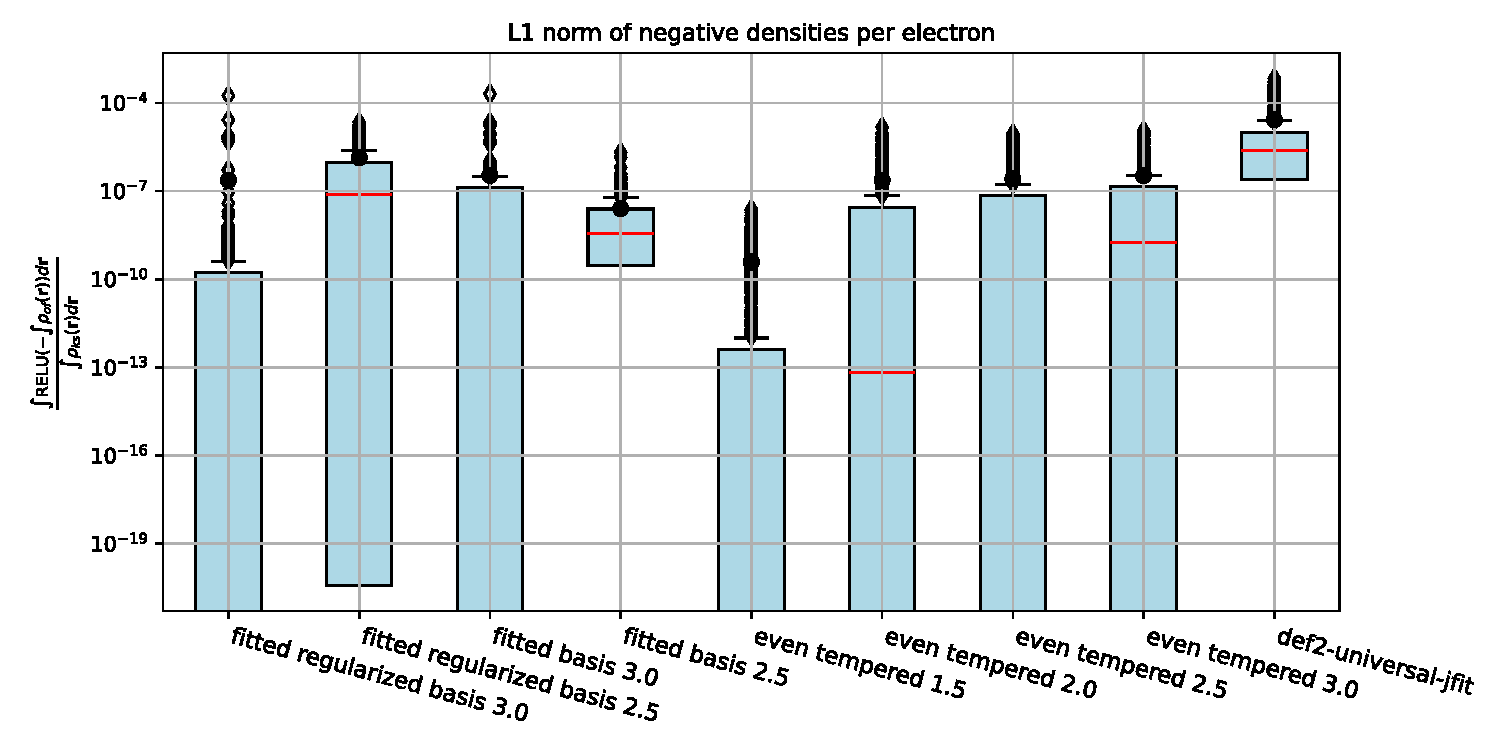
\includegraphics[width=0.9\textwidth]{chapters/results/results_images/L1_negative_densities_on_hartree+external_MOFDFT_for_different_basis_sets}
    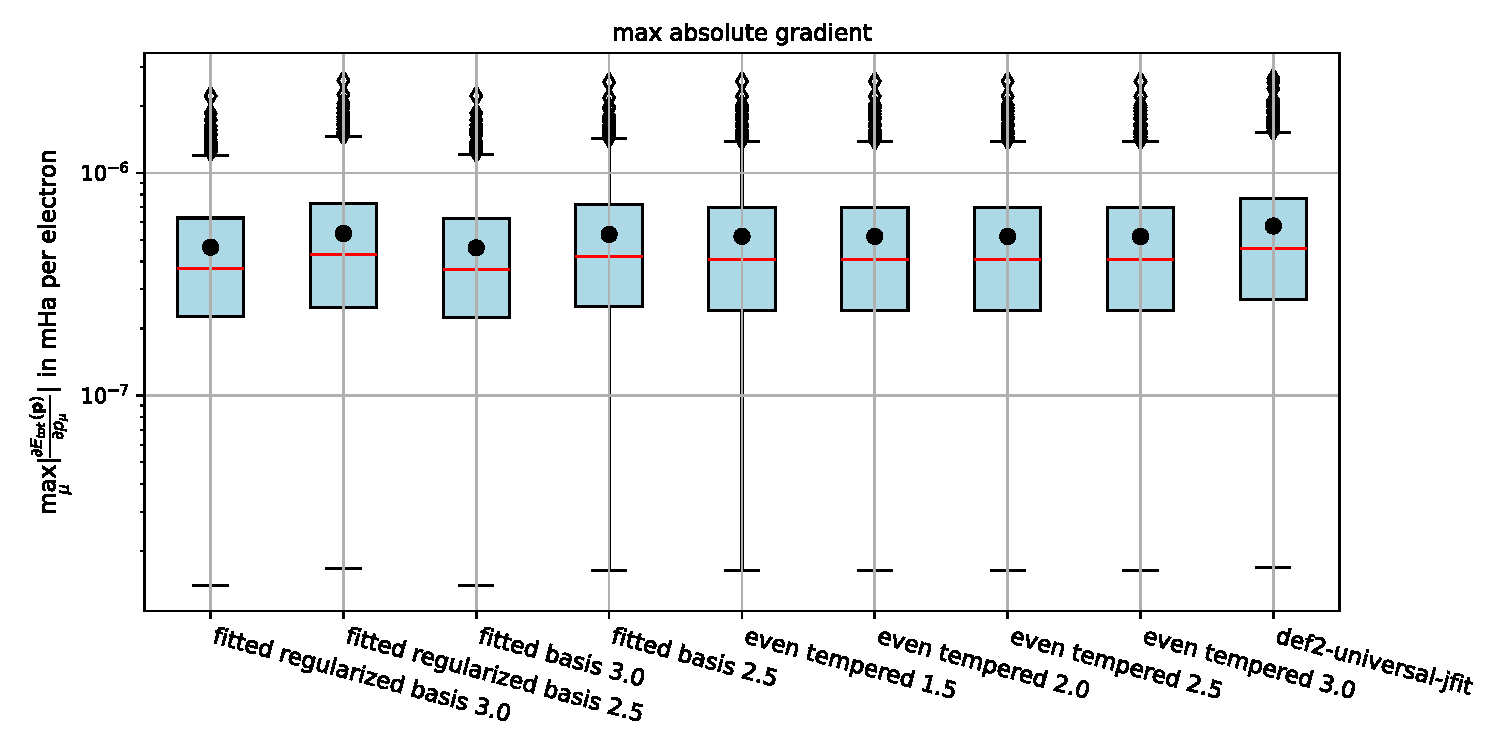
\includegraphics[width=0.9\textwidth]{chapters/results/results_images/max_abs_gradient_on_hartree+external_MOFDFT_for_different_basis_sets}
    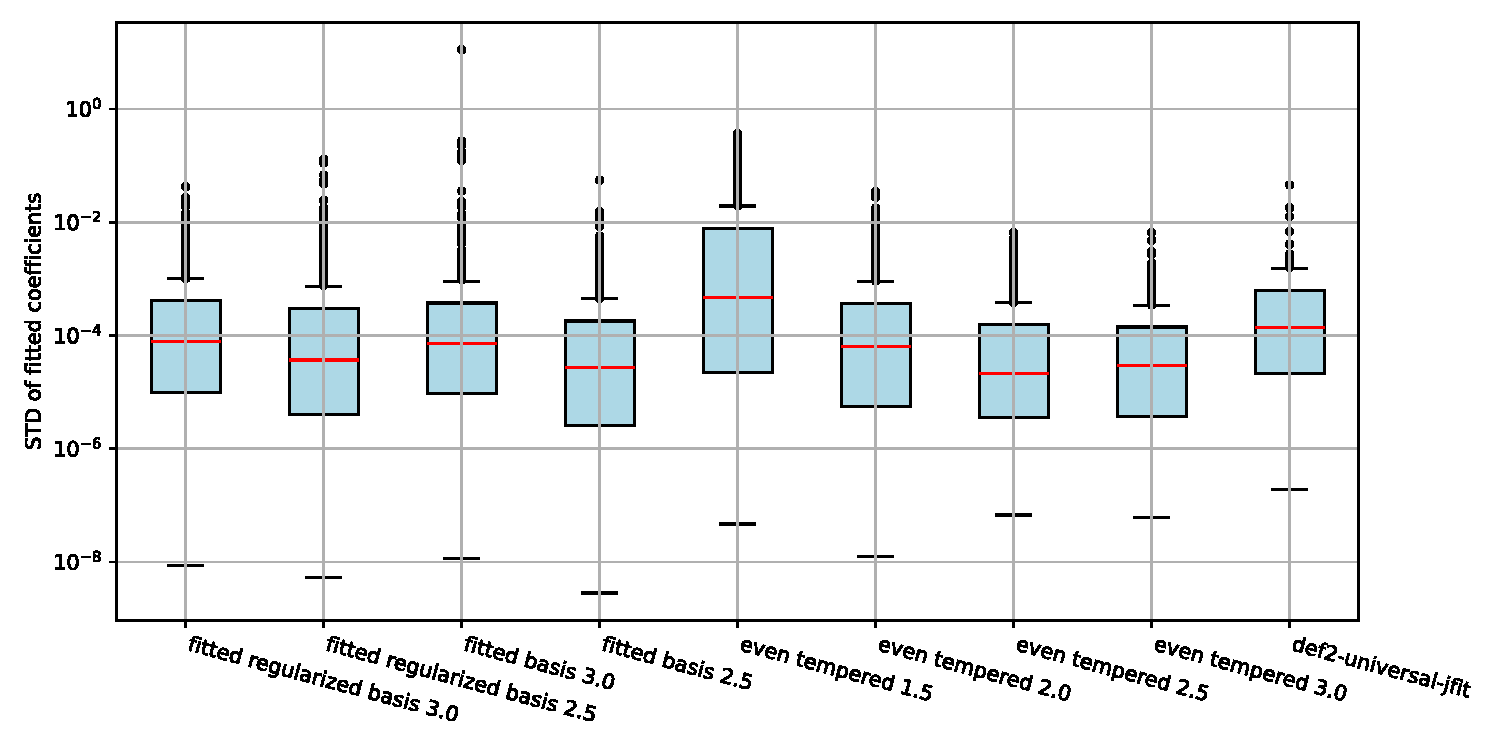
\includegraphics[width=0.9\textwidth]{chapters/results/results_images/var_basis_sets}
    \caption{Boxplots(\ref{boxplots}) analysing the different additional metrics for the fitted basis sets}
\end{figure}

\begin{figure}
    \centering
    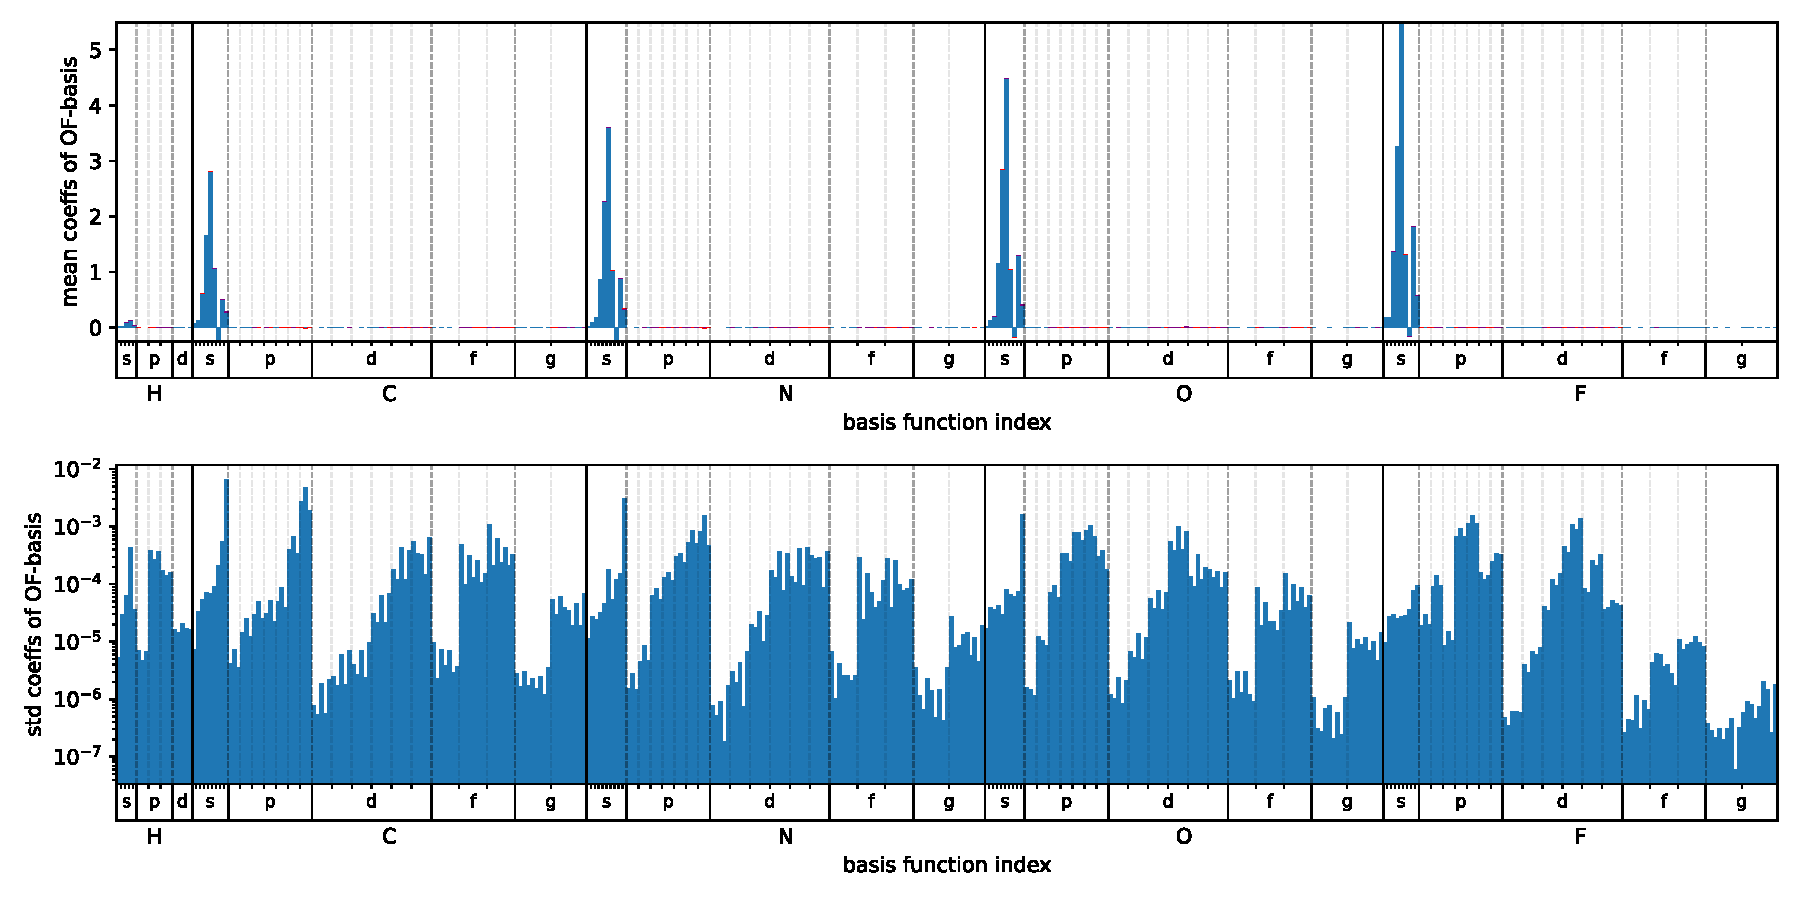
\includegraphics[width=0.9\textwidth]{chapters/results/results_images/var_coeffseven_tempered_3.0}
    \caption{The mean values(top) and the standart deviation(bottom) of the coefficients of an even tempered basis set with $\beta = 3.0$} \label{fig:var_coeffseven_tempered_3.0}
    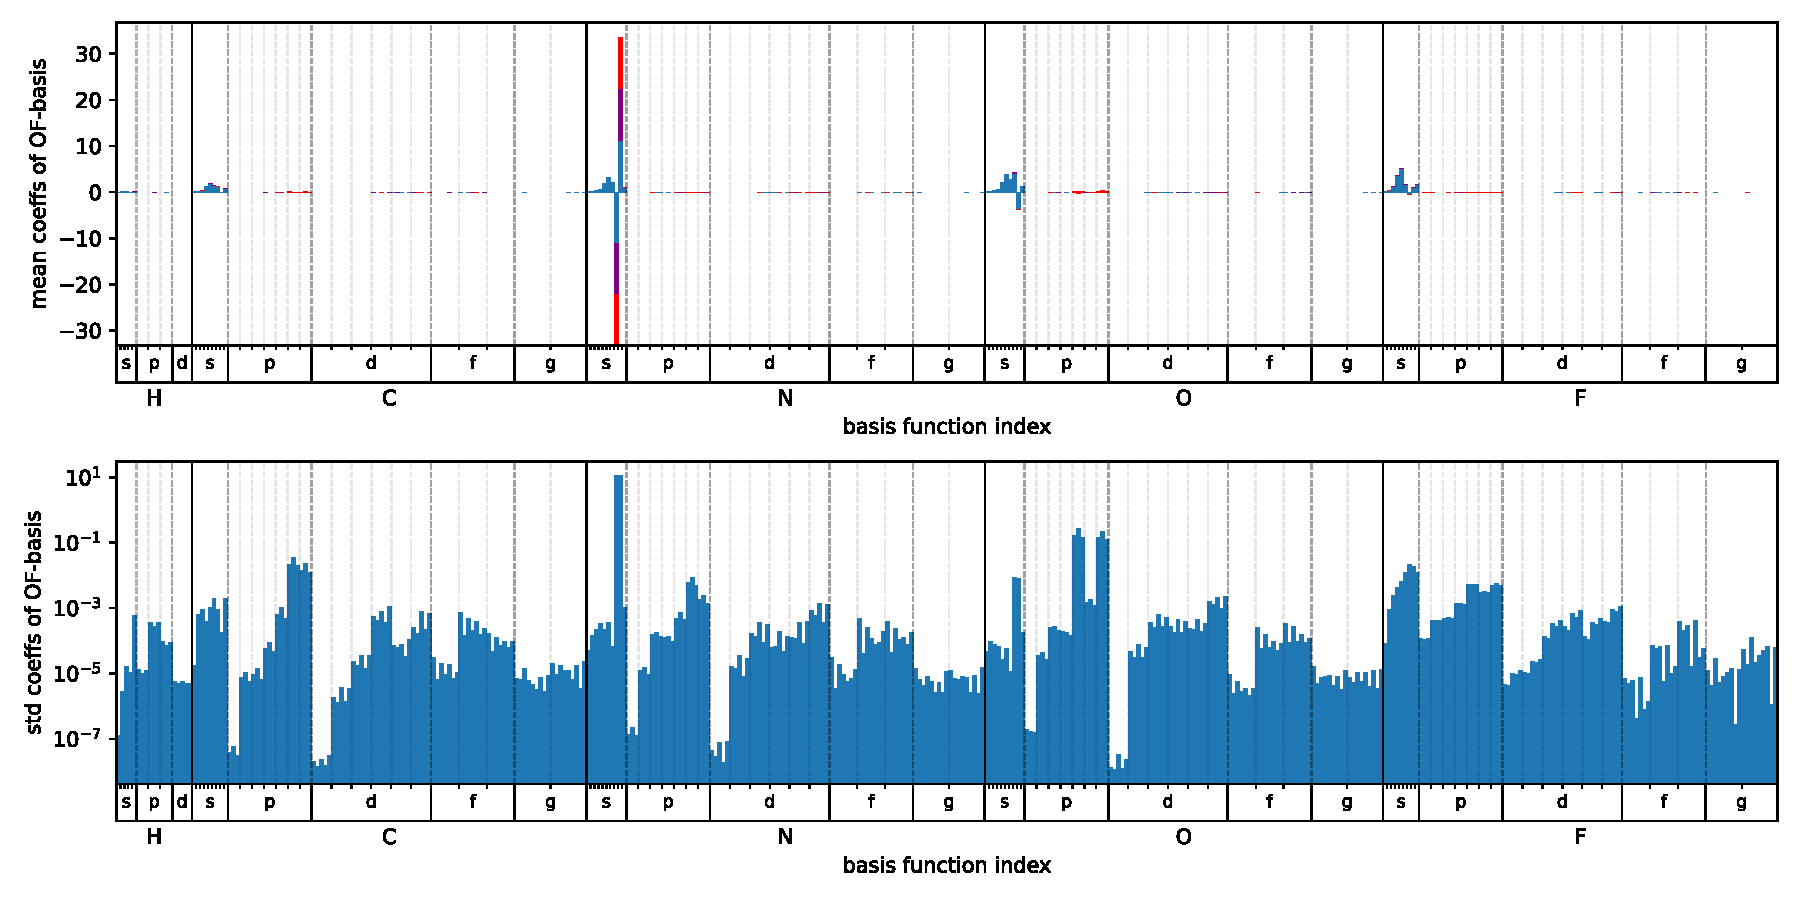
\includegraphics[width=0.9\textwidth]{chapters/results/results_images/var_coeffsfitted_basis_3.0}
        \caption{The mean values(top) and the standart deviation(bottom) of the coefficients of an basis set  fitted from even tempered with $\beta = 3.0$ without regularisation} \label{fig:var_coeffsfitted_basis_3.0}
    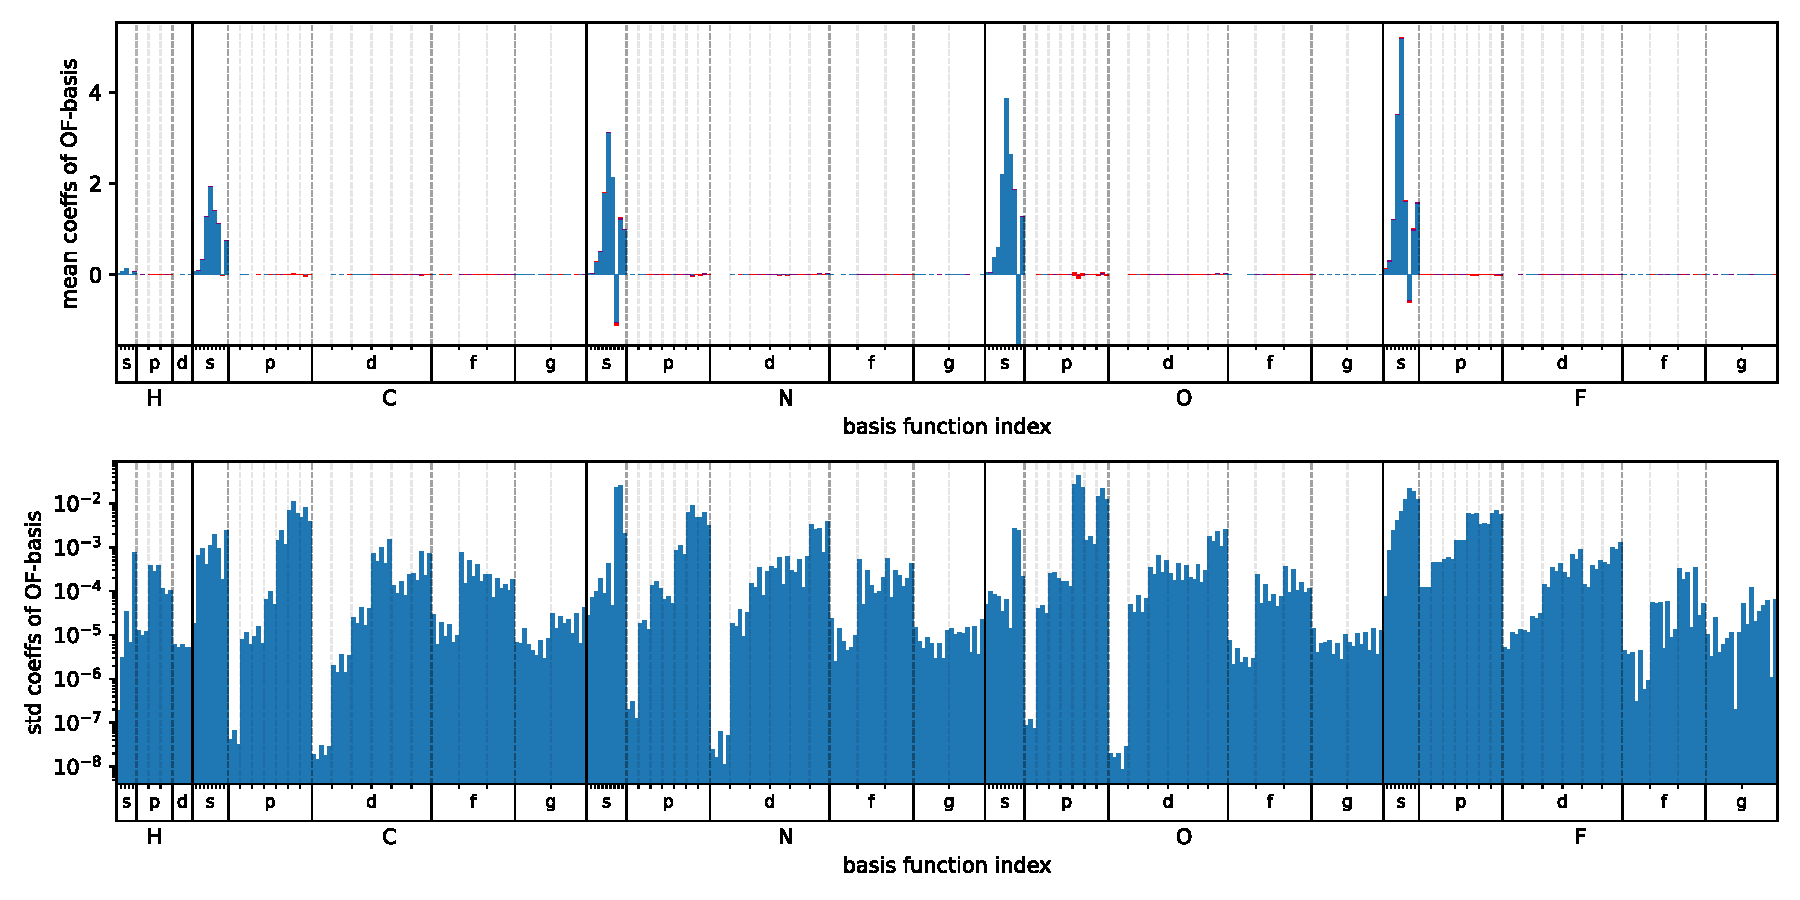
\includegraphics[width=0.9\textwidth]{chapters/results/results_images/var_coeffsfitted_regularized_basis_3.0}
        \caption{The mean values(top) and the standart deviation(bottom) of the coefficients of an basis set  fitted from even tempered with $\beta = 3.0$ after finetuning with regularisation} \label{fig:var_coeffsfitted_regularized_basis_3.0}
\end{figure}
As before, we can also examine the difference in densities directly, which are depicted in figure \ref{fig:slices_basis_sets}. Here we can rediscover our findings from the metrics. Far away from the atomic nuclei, the error in density for all tested basis sets is low compared to the error in the core regions (notice the different scales). When moving to bigger basis sets, i.e., even-tempered basis sets with a lower $\beta$, we observe that the density error in the core regions is strongly improved while the error in the outer regions is only slightly improved. The fitted basis sets also mainly improve the density near the atomic center while only minimal changes are noticeable far from the nuclei. The regularized basis sets perform slightly worse than the non-regularized basis sets. As most of the density and density fitting error is concentrated around the core, it is plausible that the loss also puts emphasis on improving the density in the center, and only when the density around the cores is very well reproduced will the further away regions be optimized. In table \ref{tab:basis-comparison-detailed}, we can also see that the bigger even-tempered basis sets improve the number of basis functions in each shell but don't add higher-order shells. If one wants to improve the density in the surrounding areas, adding basis functions with higher angular momentum could be necessary, but as there is very little density located there, the improvements would probably be minimal.\\
 \begin{figure}
   \centering
   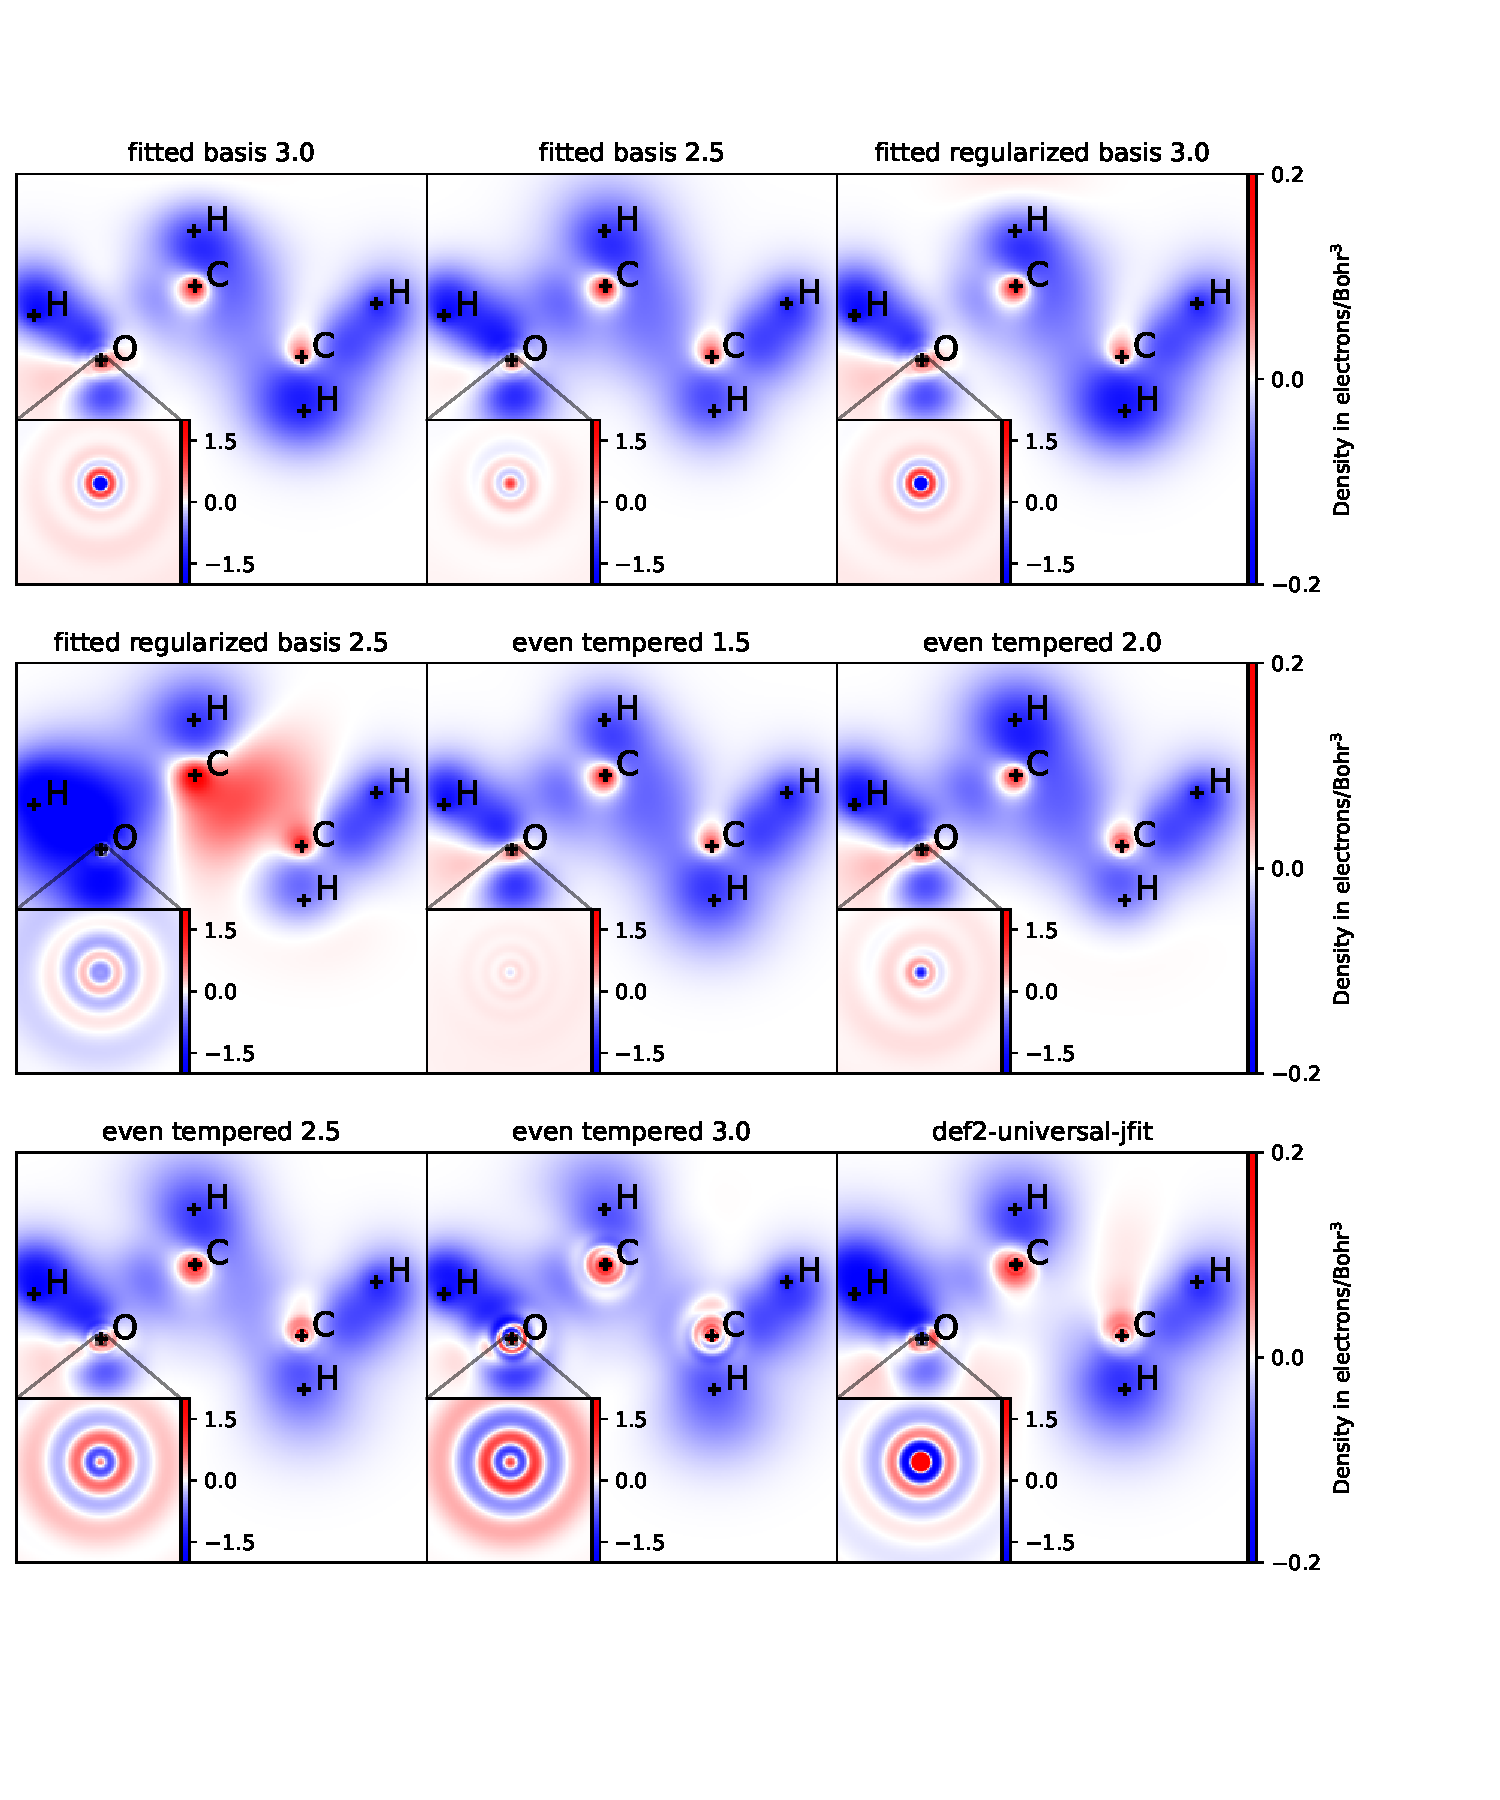
\includegraphics[width=1\textwidth]{chapters/results/results_images/basis_set_slices.pdf}
     \caption{Slices of the fitted density with density fitting method hartree+external Mofdft using different basis sets}
     \label{fig:slices_basis_sets}
 \end{figure}



\begin{figure}
   \centering
   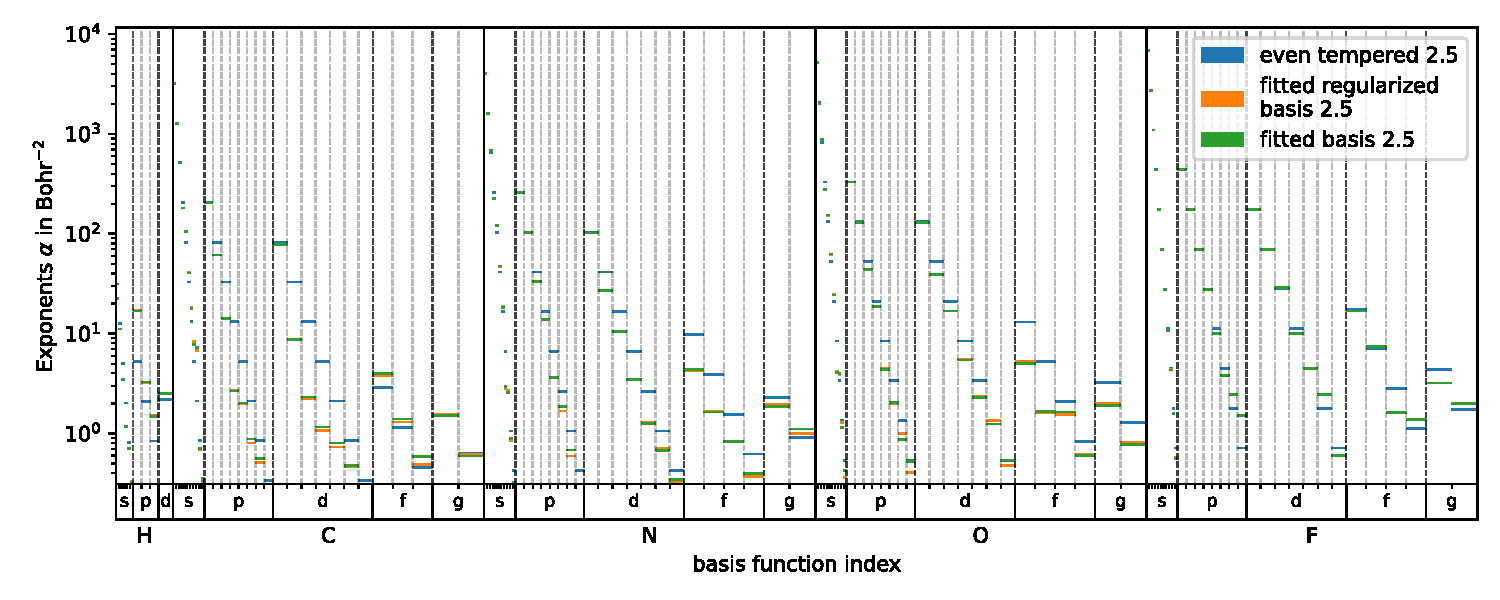
\includegraphics[width=0.6\textwidth]{chapters/results/results_images/basis_functions_with_size2.5}
   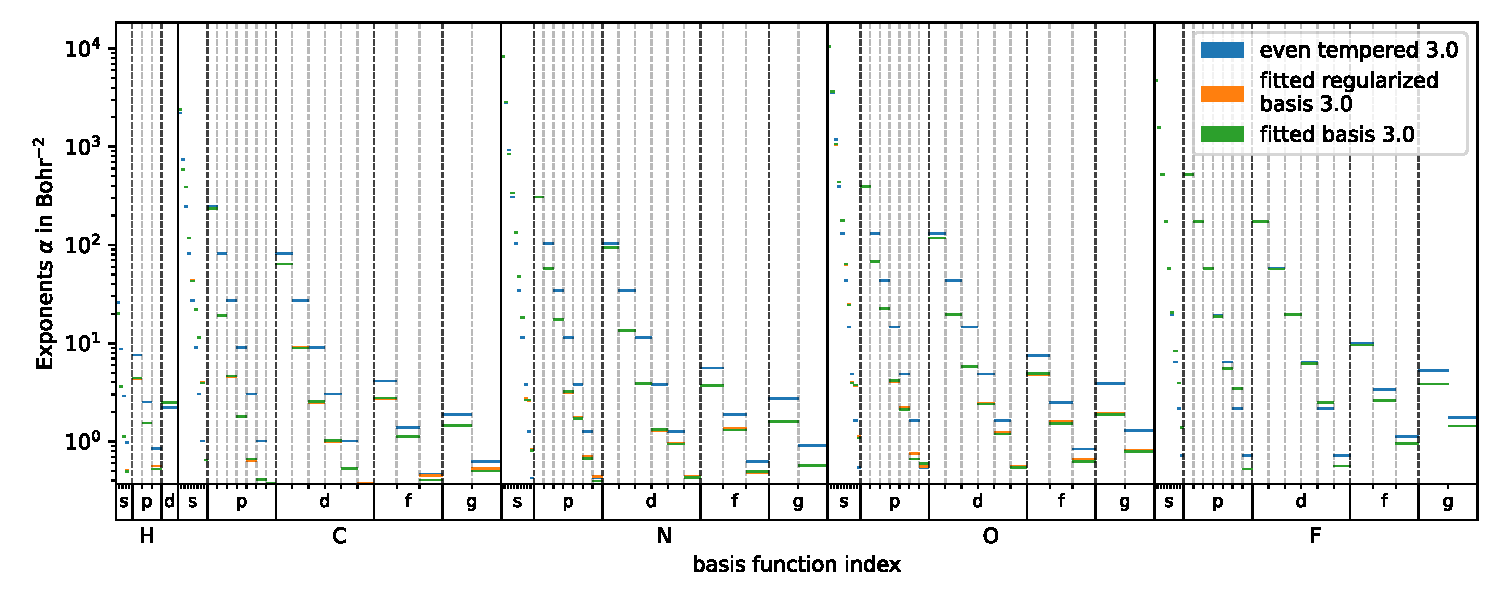
\includegraphics[width=0.6\textwidth]{chapters/results/results_images/basis_functions_with_size3.0}
    \caption{}
\end{figure}
\section{Conclusion}
To summarize our findings, we have shown that by using differentiable integrals and stochastic gradient descent, we can optimize the basis functions of an orbital-free basis set to better fit the density produced by a Kohn-Sham calculation. The fitted basis sets improve upon the standard even-tempered basis sets in both the reproduced energies and the quality of the density fit. Without regularization, the fitted basis sets tend to cluster some exponents very close together, which can lead to very large and unstable coefficients and, when employed in a machine learning context, can greatly hinder training. The regularization procedures can remove these problems but also lead to slightly worse metrics.\\
Altogether, our produced basis sets can increase the accuracy of orbital-free DFT without the need for more basis functions, which would otherwise slow training.










